%%%%%%%%%%%%%%%%%%%%%%%%%%%%%%%%%%%%%%%%%%%%%%%%%%%%%%%%%%%%%%%%%%%%%%%%%%%%%%%%
%2345678901234567890123456789012345678901234567890123456789012345678901234567890
%        1         2         3         4         5         6         7         8

\documentclass[letterpaper, 10 pt, conference]{ieeeconf}  % Comment this line out
                                                          % if you need a4paper
%\documentclass[a4paper, 10pt, conference]{ieeeconf}      % Use this line for a4
                                                          % paper

\IEEEoverridecommandlockouts                              % This command is only
                                                          % needed if you want to
                                                          % use the \thanks command
\overrideIEEEmargins
% See the \addtolength command later in the file to balance the column lengths
% on the last page of the document



% The following packages can be found on http:\\www.ctan.org
%\usepackage{graphics} % for pdf, bitmapped graphics files
%\usepackage{epsfig} % for postscript graphics files
%\usepackage{mathptmx} % assumes new font selection scheme installed
%\usepackage{times} % assumes new font selection scheme installed
\usepackage{amsmath} % assumes amsmath package installed
\usepackage{amssymb}  % assumes amsmath package installed
\usepackage{boldline}
\usepackage{array,multirow}
\usepackage{dblfloatfix} 
\usepackage{hyperref}
\usepackage{float}
\usepackage{color}
\usepackage{xfrac}
\usepackage{graphicx}
\graphicspath{ {images/} }
\definecolor{light-gray}{gray}{0.95}
\newcommand{\code}[1]{\colorbox{light-gray}{\texttt{#1}}}
\DeclareMathOperator*{\argmax}{arg\,max}
\DeclareMathOperator*{\maxU}{max}
\usepackage{makecell}
\usepackage{bbm}
\usepackage[table,xcdraw]{xcolor}
\usepackage[flushleft]{threeparttable}
\usepackage[utf8]{inputenc}
\usepackage{capt-of}


\title{\LARGE \bf
TITLE OF PAPER.
}

\author{ \parbox{2 in}{\centering Tamir Bennatan
         {\tt\small tamir.bennatan@mail.mcgill.ca\\}
         {\tt\small 260614526}}
         \hspace*{ 0.3 in}
         \parbox{2 in}{\centering Kyle Levy
         {\tt\small kyle.levy@mail.mcgill.ca\\}
         {\tt\small INSERT KYLES ID}}
         \hspace*{0.3 in}
         \parbox{2 in}{\centering Phillip R...
         {\tt\small INSERT PHILS EMAIL\\}
         {\tt\small ISERT PHILS ID}}
}


\begin{document}



\maketitle
\thispagestyle{empty}
\pagestyle{empty}


%%%%%%%%%%%%%%%%%%%%%%%%%%%%%%%%%%%%%%%%%%%%%%%%%%%%%%%%%%%%%%%%%%%%%%%%%%%%%%%%
\begin{abstract}

This is filler, so that we don't get formatting problems later when we write the abstract. This is filler, so that we don't get formatting problems later when we write the abstract. This is filler, so that we don't get formatting problems later when we write the abstract. This is filler, so that we don't get formatting problems later when we write the abstract. This is filler, so that we don't get formatting problems later when we write the abstract. This is filler, so that we don't get formatting problems later when we write the abstract. This is filler, so that we don't get formatting problems later when we write the abstract. This is filler, so that we don't get formatting problems later when we write the abstract. 

\end{abstract}


%%%%%%%%%%%%%%%%%%%%%%%%%%%%%%%%%%%%%%%%%%%%%%%%%%%%%%%%%%%%%%%%%%%%%%%%%%%%%%%%
\section{INTRODUCTION}

The MNIST dataset - comprising of images of handwritten digits of 10 classes - is a popular dataset, widely used as a  benchmark for learning and classification tasks amongst the Neural Network and Computer Vision communities. MNIST enjoys several favorable charactaristics which have contributed to its widspread adoption (Cohen, et. al; 2017). First, the dataset is relatively small (each of the 60,000 examples are $(28\text{x}28)$ pixel grayscale images), which makes it feasible to work with the dataset on most processors [Figure 1]. Second, the digits have been centered within each image, have consistent heights and similiar widths. The digits are all distinguishable to the human eye, and the labels associated with each image are accurate. Because of these properties, many reserachers have achived near perfect accuracy in the image classification task on MNIST (for example: Lecun et. al; 2001).

\begin{figure*}[ht]
\centering
\begin{minipage}{.5\textwidth}
  \centering
  
\includegraphics[width=1\linewidth]{mnist_sample}
  \captionof{figure}{Three sample images from the MNIST dataset.}
  \label{fig:test1}
\end{minipage}%
\begin{minipage}{.5\textwidth}
  \centering
  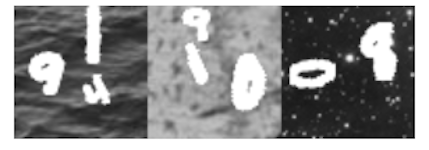
\includegraphics[width=1\linewidth]{emnist_sample}
  \captionof{figure}{Three sample images from the EMNIST dataset.}
  \label{fig:test2}
\end{minipage}
\end{figure*}

In this project, we address the digit classification task on a more difficult dataset called Extended-MNIST (EMNIST). Each example int he EMNIST daset was generated with the following procedure:
\begin{enumerate}
\item Randomly select 2 or 3 images from MNSIT.
\item Rescale each image by a factor ranging from 40\% to 120\% the original size (the label of the generated image is that of the MNIST image which was scaled up by the largest factor).
\item Apply random rotations to each image. 
\item Superimpose these rotated images onto a random background.
\end{enumerate}

The inherent randomness in the EMNIST examples makes image classification on EMNIST more difficult than on MNIST [Figure 2]. 

In this report, we discuss the pre-processing measures we took to adress the noisy features of the EMNIST examples. We then summarize our process in fitting and tuning Logistic Regression, Feedforward Neural Network, and Convolutional Neural Network (CNN) classifiers. CNNs proved most effective; we achieved \textbf{90\% IS THIS TRUE?} validation accuracy using a CNN with 6 convolutional layers. We then summarize our results and our shortcomings, and ways in which we can improve our accuracy in the future. 

\section{Feature Design}

The EMNIST dataset introduces several difficulties in building an effective classifier. The random backgrounds of each example in the EMNIST dataset were generated independently of the examles' labels. Thus, they only add noise to each image, which can impede effective learning by a machine learning algorithm. 

It is also unclear which digit in each image was scaled up the most during the construction of each example in EMNIST, as we do not have prior knowledge of the dimension sof the MNIST digits used to create each example in EMNIST. This makes it difficult to isolate the digit within each EMNIST example that corresponds with the target label.

Finally, an effective classifier for the EMNIST dataset must be robust to rotations in images, as the EMNIST datsset was built by rotating MNIST images randomly. As most machine learning algorithms do not encode images in a way that is robust to rotations, this adds diffulty to the classification task. 

\subsection{Removing Noisy Backgrounds} 

The first preprocessing step we took was to remove the backgrounds of each example in EMNIST. Luckily, the pixels in each example corresponding to a digit extracted from MNIST have a fixed integer value of 255 (corresponding to the color white). This made it possible to replace the random backgrounds with black backgrounds, by converting all non-white pixels to black pixel values [Figure 3].
\begin{figure}[H]
      \centering
      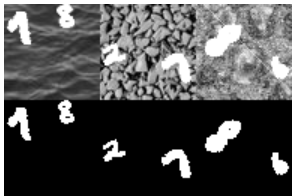
\includegraphics[scale = 1]{blackout}
		\centering
      %\includegraphics[scale=1.0]{figurefile}
      \caption{Three sample images from EMNIST, before filling the backgrounds (top) and after filling the backgrounds (bottom).}
      \label{figurelabel}
   \end{figure}

\subsection{Extracting the 'Largest' Digit} 

Each example in EMNIST contains several digits, but only one label. Intuitively, this makes the learning task difficult, as a machine learning algorithm will try associate the properties of several digits which an example's label, when in fact the task is to only correctly identify the \emph{largest} digit. 

Thus, we set out to extract the \emph{"largest"} digit from each example in EMNIST. Since we do not know the original dimensions of each of the digits in each image, we employed a series of heuristics to define the size of an digit. These heuristics are:
\begin{enumerate}
\item \textbf{Bounding Rectangle Area:} The area of the smallest upright rectangle that circumscribes the digit. 
\item \textbf{Bounding Circle Area:} The area of the smallest circle which escribes the digit. 
\item \textbf{Minimum Rotated Rectangle Area:} The area of the smallest (possibly rotated) rectangle that escribes the digit.
\item \textbf{Minimum Rotated Rectangle Maximum Dimension} The largest dimension (height,width) of the smallest (possibly rotated) rectangle that circumscribes the digit. 
\end{enumerate}
We refer to these huristics as \emph{heuristics 1-4}, respectively.

\begin{figure}[H]
      \centering
      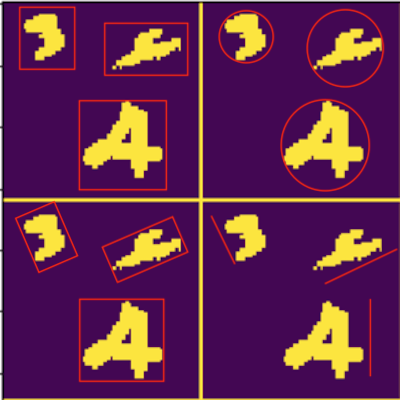
\includegraphics[scale = 1]{size_definitions}
		\centering
      %\includegraphics[scale=1.0]{figurefile}
      \caption{A sample image from EMNIST, superimposed by the geometric objects used to measure the size of each image using heuristics 1-4. Heuristic 1 is the top left, Huerustic 2 is the top right, Heuristic 3 is the bottom left, and Heuristic 4 is the bottom right.}
      \label{figurelabel}
   \end{figure}

We treated the choice of which heuristic to use to measure the size of a digit as a hyperparameter, selected from them using cross-validation. Once we selected a heuristic, cropped each example to the a square which circumscribes the largest digit (according to this heuristic), and resized this square to 28 by 28 pixels. 

\subsection{Data Augmentation} 

To help make our model more robust to rotated digits, we augmented our training data with randomly rotated copies of each training example. Our rational is that if we train on randomly rotated images, our classifier will scale unseen randomly rotated images more effeciely. We tuned the number of times we rotated each image (called the \emph{"batch size"}), and the range of degrees with which we rotated each image as hyperparameters. 

\begin{figure}[H]
      \centering
      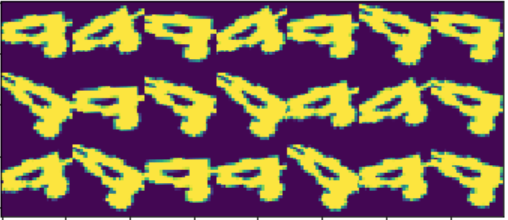
\includegraphics[scale = .7]{rotated_nines}
		\centering
      %\includegraphics[scale=1.0]{figurefile}
      \caption{21 images generated from one digit extracted from an EMNIST example via random rotations. These images can be used to augment the training data.}
      \label{figurelabel}
   \end{figure}


\section{Algorithms}

We trained classifiers of three types: Regularized Logistic Regression, Feedforward Neural Network, and Convolutional Neural Networks (CNN). We trained each of these classifiers on the datasets processed using each of size heuristics described above, though we only experimented with data augmentation when training the CNN.

Regularized Logisitc regression served as our benchmark, as it is a simple and easy to implement algorithm. The two hyperparamters we tuned (besides the chosen size heuristic) were the inverse-regularization coefficient, $C$\footnote{In the notation seen in class, $C \equiv \sfrac{1}{\lambda}$.}, and the regularization loss function (either \emph{l1} or \emph{l2} loss). 

\textbf{THIS IS FILLER. HERE WE TALK A BIT ABOUT IMPLEMENTATION AND WHAT WE TUNEDTHIS IS FILLER. HERE WE TALK A BIT ABOUT IMPLEMENTATION AND WHAT WE TUNEDTHIS IS FILLER. HERE WE TALK A BIT ABOUT IMPLEMENTATION AND WHAT WE TUNEDTHIS IS FILLER. HERE WE TALK A BIT ABOUT IMPLEMENTATION AND WHAT WE TUNEDTHIS IS FILLER. HERE WE TALK A BIT ABOUT IMPLEMENTATION AND WHAT WE TUNEDTHIS IS FILLER. HERE WE TALK A BIT ABOUT IMPLEMENTATION AND WHAT WE TUNEDTHIS IS FILLER. HERE WE TALK A BIT ABOUT IMPLEMENTATION AND WHAT WE TUNED.}


\subsection{Baseline Features and Models} 

We built a baseline feature set and model so that we could measure the relative increase in performance that results from incorporating each new feature set.

Our baseline feature set consists of standard syntactic and string edit distance features\footnotemark . We also noticed that many Kaggle competitors used neural word embeddings to construct “sentence vectors” for each question by averaging the embedding vectors of each word in a question. They then used various similarity functions\footnotemark \ to compute the similarity between the sentence vectors of paired questions as features. We recreated these features using the fastText pre-trained word embeddings (Joulin et al.; 2016). Our initial features are summarized in Table 2.

\begin{table}[b]
\centering
\caption{Baseline features}
\label{my-label}
\begin{tabular}{|p{15mm}|p{60mm}|}
\hline
Feature \\ category                          & Feature \\ \hlineB{3}

Syntactic                        & Number of words in each question \\\cline{2-2}
features							   & Number of words the two questions have in common \\\hline

Character 				   & Number of characters in each question \\\cline{2-2} 
 	features						   & Difference in number of characters in each question \\
\hline

Edit  		   & 	Partial string matches (with/without stopwords)			\\\cline{2-2}
distance 	& Token-wise string matches \\\cline{2-2}
variations 	 				& Type-wise string matches \\\cline{2-2}
 								& Type-sorted string matches \\

\hline

Sentence embedding similarity	   & Vector similarities of sentence embeddings using Euclidean, Cosine, Cityblock, Bray-Curtis and Jaccard distances\\ 
				   	
\hline

\end{tabular}
\end{table}





We then split the dataset into training and test splits, which we kept consistent in all further experiments. 
We trained logistic regression and gradient boosted trees (XGB) models on the training set using the features described in Table 2, and used 3-fold cross validation to tune hyperparameters. These are our baseline features. 

To test whether logistic regression and XGB are adequate models for this task, we also implemented an LSTM classifier, since many Kaggle competitors demonstrated that these models perform well on the Quora dataset. With the use of a development set, we compared several LSTM architectures, and found that the Manhattan Siamese LSTM (MaLSTM) architecture (Mueller et al; 2016) performed best. 


\footnotetext[1]{Edit distance variations were computed using the Python \emph{fuzzywuzzy} package. More information on these metrics can be found \href{http://chairnerd.seatgeek.com/fuzzywuzzy-fuzzy-string-matching-in-python/}{\color{blue} here.}}

\footnotetext[2]{Vector similarities were calculated using the Python \emph{SciPy} package. More information on these metrics can be found \href{https://docs.scipy.org/doc/scipy/reference/spatial.distance.html}{\color{blue} here.}}

The MaLSTM is a Siamese neural network which forms a prediction by taking the Manhattan Similarity of of the vector representations of two inputs where the Manhattan similarity of two vectors $v_1$ and $v_2$ is defined:
$$
    ManhattanSim(v_1, v_2) = \exp(-||{v_1 - v_2||_1})  \eqno{(1)}
$$
We used fastText word embeddings of the words in each question as inputs to the MaLSTM. More details on our chosen architecture can be found in Appendix 1. 

We found that the XGB model, when trained on the baseline features, had performance similar to that of the MaLSTM. Thus, we concluded that the XGB model has the capacity to achieve satisfactory results in the question duplicate detection task. 

\subsection{Tf-Idf Features}


Suppose we were allowed to compare only one word from each question in a pair to determine if the questions are duplicates, but had a choice of which words to compare. Which words should we choose? We would reasonably want to choose the most \emph{important} word from each question, or the words which are most particular to each question. 

For example, in the fabricated question pair:
\begin{enumerate}
\item \emph{Who is the president of the United States?} 
\item  \emph{What is the highest paying government position?}
\end{enumerate}
We would probably derive more insight into the similarity/dissimilarity of these questions by analyzing the words \emph{president} and \emph{government} than if we compared more commonly occurring words, like \emph{who} and \emph{highest}.

We capture this intuition by creating a set of features that incorporate the Tf-Idf scores of each word. We used Scikit-Learn’s \code{TfidfTransformer} class  (Pedregosa et al.; 2011) to compute the Tf-Idf of a word $w$ in document $d$ using the formula:

$$
Tf\text{-}Idf(w, d) = Tf(w,d) * Idf(w) \eqno{(2)}
$$
Where $Tf(w,d)$ is the number of times word $w$ appers in document $d$ (term frequency), and $Idf(w)$ is defined:
$$
Idf(w) = \log{\frac{1 + n_d}{1 + df(w)}} + 1  \eqno{(3)}
$$
Where $n_d$ is the number of documents\footnote{\emph{Documents} and \emph{texts} are questions, in this context.} in the corpus, and $df(w)$ is the number of documents in the corpus that contain the word $w$. 

The Tf-Idf weight of a word in a document will be high if: 1) the word appears many times in  that document, and 2) the word has low document frequency. It serves as a natural heuristic for modelling the relative importance of a word within a document. Tf-Idf weights are useful for many NLP tasks; in fact, variations of this scoring scheme are used as term weights in nearly all vector space information retrieval models (Jurafsky \& Martin; 2012). 

Thus, we used Tf-Idf scores to craft four new features. The first two attempt to measure similarity of the “most important” word of each question in a pair. To do so, we find the word with the highest Tf-Idf weight in each question, then take the fastText word embedding for each of these words, and compute the distance between these vectors. We used Euclidean distance for one feature and Cosine distance for the second.

$$
{Feature}_1 = ||Embed(w_1^*) - Embed(w_2^*)||_2 \eqno(4)
$$
$$
{Feature}_2 = \frac{\langle Embed(w_1^*), Embed(w_2^*) \rangle}{||Embed(w_1^*)||_2||Embed(w_2^*)||_2} \eqno(5)
$$
Where
$$
w_i^*= \argmax_{w_i \in d_i} \{ {Tf\text{-}Idf(w_i, d_i)}\} \quad \quad \quad  i \in \{1,2\}
$$

The third and fourth features measure the total Tf-Idf weight of the words two questions have in common, and the total weight of the words that they don’t: 

$$
{Feature}_3 = \sum_{w \in \{d_1 \cap d_2\}}{Tf\text{-}Idf(w, \{d_1 \cap d_2\})} \eqno(6)
$$
$$
{Feature}_4 = \sum_{w \in \{d_1 \bigtriangleup  d_2\}}\sum_{i = 1}^2{Tf\text{-}Idf(w, d_i)\mathbbm{1}(w \in d_i) } \eqno(7)
$$

\subsection{Question Classifcation Features}

IR-based question answering (QA) systems attempt to find short segments of text that answer a user’s question by querying a database or searching the web (Jurafsky \& Martin; 2017). These systems tend to perform better if they first constrain the answer candidates using a semantic categorization of the expected answer of an input question (Li \& Roth; 2002).  

For example, when considering the question:
\begin{center}
\emph{Who is the president of the United States?}
\end{center}
A QA system should limit its search to words that correspond to humans, as opposed to considering all noun-phrases.

Using the Text Retrieval Conference (TREC) question dataset (Voorhees; 2002), Roth and Li (2005) developed a hierarchical taxonomy for classifying the answer type of a question. This taxonomy consists of 6 coarse categories, and 50 fine sub-categories. They then annotated the 6000 questions in the TREC dataset using this taxonomy. The coarse answer categories are LOCATION, DESCRIPTION, ENTITY, NUMERIC, HUMAN, and ABBREVIATION, and some examples of fine categories are NUMERIC::Date and NUMERIC::Money. The task of predicting the answer type of a question is broadly termed \emph{Question Classification}. 

We hypothesized that knowing the answer types of the questions in the Quora dataset would be useful for the question duplicate detection problem, since two questions are more likely to have duplicate intent if they share the same answer type. Our next feature set tests this hypothesis. 

We trained 5 LSTM models on the TREC dataset to predict the coarse categories of each question. These models each have slightly different architectures, but they all consisted of three layers:
\begin{enumerate}
\item Embedding layer using pretrained fastText 300-dimensional embeddings
\item LSTM layer of output dimension 50
\item Output layer (of varying types) of output dimension 6.
\end{enumerate}
The details of the different architectures are in Table 3. Note that we trained these LSTMs on the entire TREC dataset without the use of the development set,  so we make no statement about the efficacy of these models for question classification.


\begin{table}[]
\centering
\caption{Architecture details of LSTM question classifiers }
\label{my-label}
\begin{tabular}{|p{10mm}|p{10mm}|p{10mm}|p{10mm}|p{14mm}|p{8mm}|}
\hline
Model  & Output Layer & Dropout  & Recurrent Dropout & Embeddings Trainable? & Input Length \\ \hline
LSTM 1 & Dense             & 20\%                   & -                 & NO                    & 10           \\
LSTM 2 & Dense             & -                      & 20\%              & NO                    & 10           \\
LSTM 3 & LSTM              & -                      & 20\%              & NO                    & 10           \\
LSTM 4 & LSTM              & 20\%                   & 20\%              & YES                   & 10           \\
LSTM 5 & LSTM              & -                      & 20\%              & NO                    & 6            \\ \hline
\end{tabular}
\end{table}

Using these models, we predicted the answer type of the questions in the the Quora dataset. Then, considering each LSTM model separately, we added these predictions to our baseline features, and measured the increase in our baseline XGB model using 3-fold cross validation. We also tried an ensembled approach, where the predicted class of each question is the class most predicted amongst the 5 LSTMs.

We found that the ensembled predictions, as well as a binary feature which indicates if these predictions coincide, increased the performance of our baseline XGB model the most (in terms of reduction of log-loss). Thus, these are the features in the second feature set which we propose: 
$$
Feature_5 = \text{\{Question 1 Answer Type Prediction\}}
$$
$$
Feature_6 = \text{\{Question 2 Answer Type Prediction\}}
$$
$$
Feature_7 = \mathbbm{1}(\text{Answer Type Predictions Agree?})\quad
$$
\subsection{Sentence Semantic Similarity Scores}

Our final feature set uses a framework for measuring the semantic similarity of short texts proposed by Mihalcea et al (2006). This framework models the similarity of two texts as a function of the similarities of their component words and the specificity of each word. Word-to-word similarities are measured with respect to a semantic knowledge base (e.g. WordNet.)

Given a word-to-word similarity metric, $Sim(w_1, w_2)$, and two texts\footnotemark[3] $T_1,$ $T_2$, the semantic similarity score of these two texts is computed by:
\begin{enumerate}
\item For each word $w \in T_1$, find the word $w^* \in T_2$ which maximizes $Sim(w, w^*)$.
\item Apply this same process to determine the words in $T_1$ that have the highest similarity to the words in $T_2$. 
\item Sum up the similarities (weighted by a measure of specificity, such as $Idf$ $(3)$), and normalize for the length of the sequences. 
\end{enumerate}
Note that words in one text are only compared to words in the other text \emph{of the same part of speech}, as many knowledge-based similarity measures cannot be applied across parts of speech (Mihalcea et al; 2006).

\begin{gather*} \tag{8}
SimText(T_1,T_2) = \\ \frac{1}{2}\Big( \frac{\sum_{w \in T_1}{\maxU_{w^* \in T_2}Sim(w,w^*)Idf(w)}}{\sum_{w \in T_1}Idf(w)} \\ + \frac{\sum_{w \in T_2}{\maxU_{w^* \in T_1}Sim(w,w^*)Idf(w)}}{\sum_{w \in T_2}Idf(w)} \Big)
\end{gather*}
This framework guarantees the convenient properties of symmetry: $SimText(T_1, T_2)$ = $SimText(T_2, T_1)$, and that the range of the text similarity scores is the same as that of the word-to-word similarity measure  $Sim(w_1, w_2)$ used. 

We used the python NLTK package for part-of-speech tagging (Bird et al; 2009). We implemented this framework using three similarity metrics available via NLTK’s WordNet interface - path similarity, Leacock-Chodorow similarity (Leacock \& Chodorow; 1998) and Wu-Palmer similarity (Wu \& Palmer; 1994). 

We also implemented a simplified version of this framework by removing the dependency on $Idf$ scores in (8):

\begin{gather*} \tag{9}
SimText_{simplified}(T_1,T_2) = \\ \frac{1}{2}\Big( \frac{\sum_{w \in T_1}{\maxU_{w^* \in T_2}Sim(w,w^*)}}{|T_1|} \\ + \frac{\sum_{w \in T_2}{\maxU_{w^* \in T_1}Sim(w,w^*)}}{|T_2|} \Big)
\end{gather*}
We made this simplification to reduce the correlation between these similarity scores and the Tf-Idf features proposed in section 4.B - which also depend on Idf scores.

We also extended this model by using a word-to-word similarity scores based neural word embeddings. Using pre-trained GloVe word embeddings (Pennington et al.; 2014) available through the SpaCy Python package, we used the cosine similarity (5) of the embeddings of two words as the similarity function $Sim(w_1,w_2)$ in (8) and (9). 

Using 3-fold cross validation, we added different subsets of these text-to-text similarity scores to our baseline feature set, and studied resulting boost in our baseline XGB model performance. Since the text-to-text scores are highly correlated when using path similarity, Leacock-Chodorow similarity and Wu-Palmer similarity as $Sim(w_1, w_2)$, we only tested one of these scoring functions at a time. 

We found that including two semantic similarity scores, calculated using the simplified scheme (9) and using Leacock-Chodorow distance and embedding Cosine distance as $Sim(w_1, w_2)$, resulted in the largest increase in performance in our baseline model. These two similarity scores define the final feature set we propose. 

\begin{gather*} \tag{10}
Feature_{8} = \{SimText_{Simplified}(T_1, T_2) \\ \text{where } Sim(w_1, w_2) \equiv \text{Leacock-Chodorow Similarity}\}
\end{gather*}
\begin{gather*} \tag{11}
Feature_{9} = \{SimText_{Simplified}(T_1, T_2) \\ \text{where } Sim(w_1, w_2) \equiv \text{Cosine Distance (GloVe Embeddings)}\}
\end{gather*}


\section{RESULTS}

To measure the importance of each of these feature sets, we trained logistic regression and XGB models on all the features described above. We then removed different subsets of Tf-Idf, question classification and semantic scoring feature sets, and re-tuned each model's hyperparameters using 3-fold cross validation. We then used these models to predict test-set labels. The prediction accuracy for the resulting models are summarized in Table 4, as well as those of our baseline classifiers described in section 4.A. We limit our analysis to the XGB model, as this performed much better than logistic regression. 

% Please add the following required packages to your document preamble:
% \usepackage[table,xcdraw]{xcolor}
% If you use beamer only pass "xcolor=table" option, i.e. \documentclass[xcolor=table]{beamer}
\begin{table*}[]
\centering
\caption{Test set accuracy scores, with different feature sets omitted}
\label{my-label}
\begin{threeparttable}
\begin{tabular}{|
>{\columncolor[HTML]{EFEFEF}}l |c|c|c|c|c|c|c|c|}
\hline
\multicolumn{9}{|c|}{\cellcolor[HTML]{ECF4FF}XGB  AND LOGISTIC REGRESSION, WITH FEATURE SETS OMITTED}                                                                                                                                                                \\ \hline
Feature sets ommited                                                            & $\emptyset$    & \{1\}                & \{2\}                & \{3\}                & \{1,2\}       & \{1,3\}                       & \{2,3\}                      & \{1,2,3\}     \\ \hline
XGB Test Set Accuracy                                                           & \textbf{.7925} & .7624 (.0301)        & .7861 (.0064)        & .7825 (.01)          & .7585 (.034)  & .7504 (.0421)                 & .7794 (.0131)                & .7456 (.0469) \\ \hline
\begin{tabular}[c]{@{}l@{}}Logistic Regression\\ Test Set Accuracy\end{tabular} & \textbf{.6962} & .6838 (.0124)        & .6951 (.0011)        & .6837 (.0125)        & .6836 (.0126) & .6743 (.0219)                 & .6827 (.0125)                & .6728 (.0234) \\ \hline
\multicolumn{9}{|c|}{\cellcolor[HTML]{ECF4FF}BASELINE MODELS}                                                                                                                                                                                                        \\ \hline
\multicolumn{1}{|c|}{\cellcolor[HTML]{EFEFEF}Manhattan LSTM}                    & .7588          & \multicolumn{3}{c|}{\cellcolor[HTML]{EFEFEF}Human (400 Responses)} & .8175         & \multicolumn{2}{c|}{\cellcolor[HTML]{EFEFEF}Random Guessing} & .5015         \\ \hline
\end{tabular}
\begin{tablenotes}
\item Here, \{1\} are the Tf-Idf features from 4.B, \{2\} are the question classification features from 4.C, and \{3\} are the semantic similarity scores from 4.D.
\item Cells contain each model's prediction accuracy, as well as the difference between prediction accuracy and the best model's prediction accuracy. 
\end{tablenotes}
\end{threeparttable}
\end{table*}

\begin{figure*}[t]
\centering
\begin{minipage}{.5\textwidth}
  \centering
  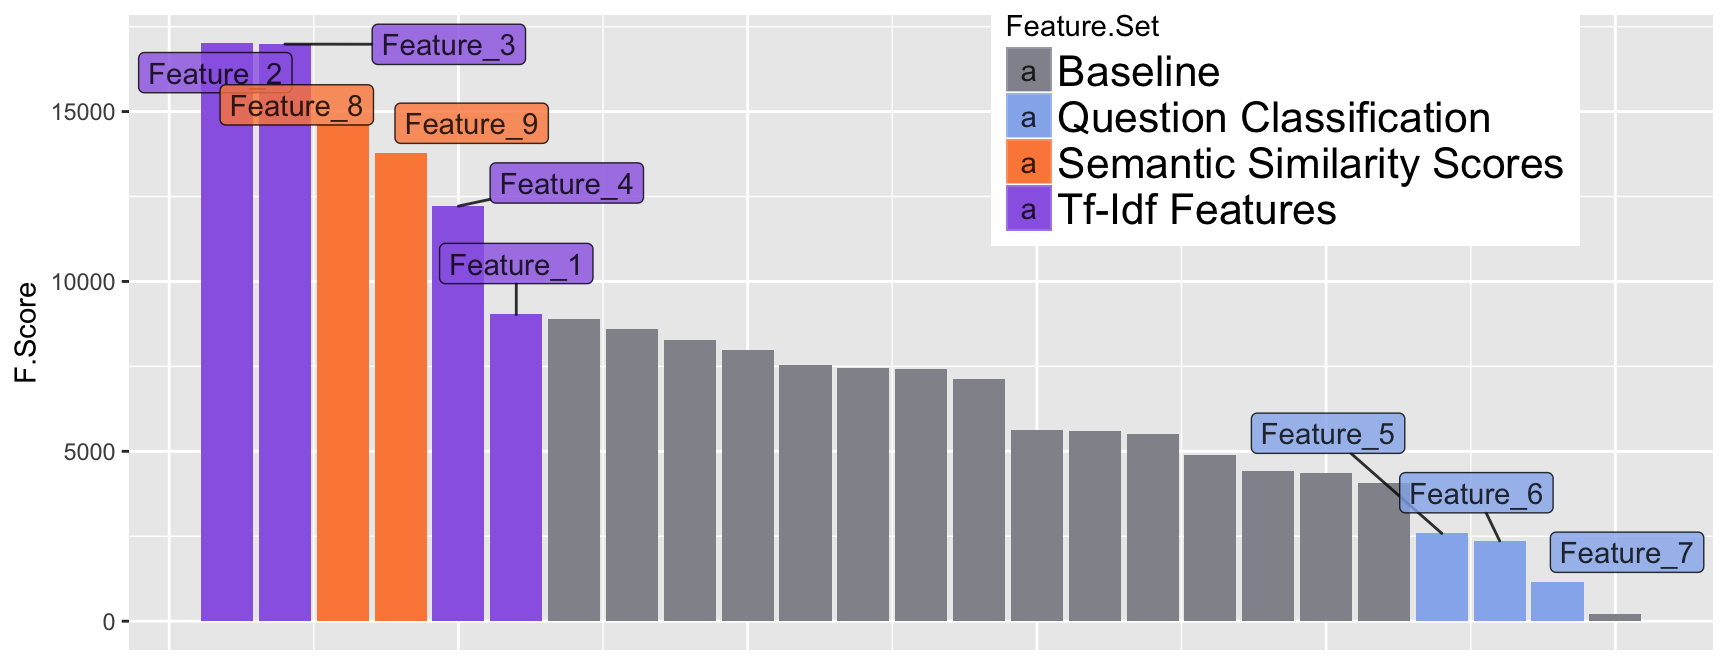
\includegraphics[width=1\linewidth]{full_bars}
  \captionof{figure}{Variable importance chart of model trained on all features.}
  \label{fig:test1}
\end{minipage}%
\begin{minipage}{.5\textwidth}
  \centering
  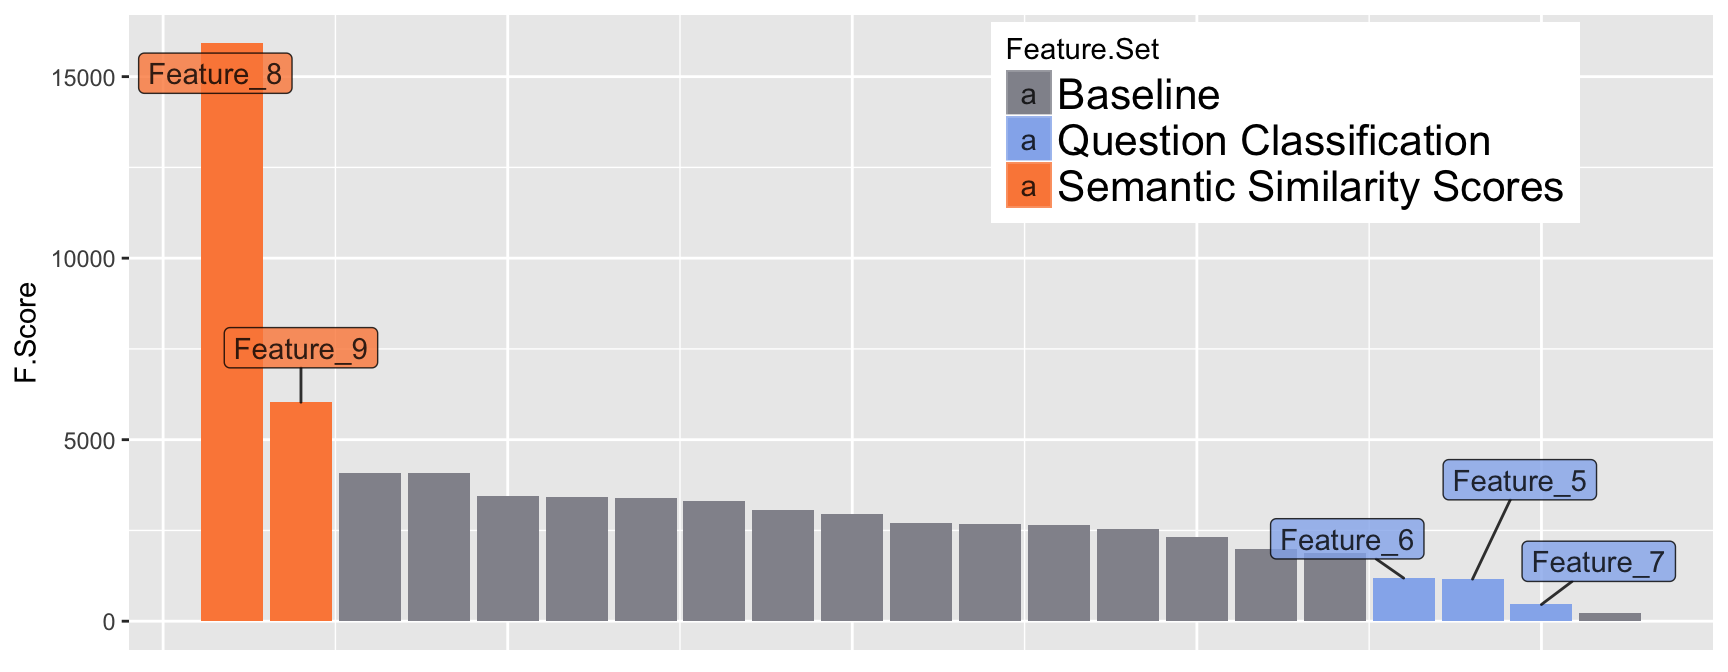
\includegraphics[width=1\linewidth]{no_tfidf_bars}
  \captionof{figure}{Variable importance chart of model that excludes the Tf-Idf features.}
  \label{fig:test2}
\end{minipage}
\end{figure*}

Including all three feature sets results in the best performance, with a test set accuracy of 79.25\% - 4.69\% better than the baseline XGB model. Amongst the three feature sets we propose, removing the Tf-Idf features (4.B) results in the largest decrease in prediction accuracy relative to the full model - with a 3.01\% decrease. Removing the question classification features from 4.C results in the smallest decrease in prediction accuracy, indicating that these features are the least meaningful of those we propose. 

When using ensembled tree models such as XGB, one can use the number of times a variable is split upon as a measure of that variable's importance. This measure is called the \emph{F-Score}. By plotting the F-Scores of each feature, we can gain insight into the importance of each variable used in a model, relative to the other variables present (Gareth et al; 2017).

A variable importance chart of the full model corroborates the result that the Tf-Idf features are the most meaningful, as these features are amongst those with the highest F-Scores [figure 1]. Semantic similarity scores also have high F-Scores. Interestingly, when the Tf-Idf features are removed, the semantic similarity scores become much more important relative to the remaining features, evident in Figure 2. This suggests that the Tf-Idf features and semantic similarity scores explain some of the same variance, and once the Tf-Idf features are removed the model must rely more heavily on the semantic similarity scores. Indeed, the features in these to feature sets are strongly correlated; the correlation between Feature 9 and Features 6 and 7 are 68.28\% and -73.91\%, respectively. 

The variable importance charts also suggest that the question classification features are not meaningful. In fact, these three features are amongst four features with the lowest F-Score.


\section{DISCUSSION AND CONCLUSIONS}

Using the three sets of features described in this paper, we were able to improve the accuracy of our baseline model from 74.56\% to 79.25\%. Of the three feature sets, those computed using Tf-Idf scores were the most impactful. This confirms our hypothesis that measures of word importance and specificity are useful in comparing the semantic similarity between two questions. 

We also applied and extended a framework for modelling semantic similarities between short texts using knowledge-based word similarity scores, proposed by Mihalcea et al (2006). We found that these scores were useful in our classification task. These features were highly correlated with those calculated using Tf-Idf scores, so it may be that they are merely capturing the specificity of the words in each question, rather than the semantic similarity of these words. 

Finally, we found that our answer type predictions were not useful for detecting duplicate questions. We suspect that this is because we used overly complex models to predict the answer type of a question. The TREC dataset has only 6,000 observations, but the number of parameters in our LSTM classifiers ranged from 70,506 to 28,141,268. It's probable that these classifiers were overfit to the TREC dataset, and did not generalize to the Quora dataset. 

In future work, we would like to try using simpler models for predicting a question's answer type - such as Naïve Bayes or a Support Vector Machine. We could also try to incorporate predictions of the fine answer categories in the annotated TREC dataset, as apposed to the coarse categories we used. 

We also think that an interesting extension to this work would be to extract features that concern the grammatical functions of the words in each question. For example, one could construct a dependency parse tree for each question, and compare the subjects and  direct objects in each question, as well as the head words of their repsective parses.

\addtolength{\textheight}{-12cm}   % This command serves to balance the column lengths
                                  % on the last page of the document manually. It shortens
                                  % the textheight of the last page by a suitable amount.
                                  % This command does not take effect until the next page
                                  % so it should come on the page before the last. Make
                                  % sure that you do not shorten the textheight too much.

%%%%%%%%%%%%%%%%%%%%%%%%%%%%%%%%%%%%%%%%%%%%%%%%%%%%%%%%%%%%%%%%%%%%%%%%%%%%%%%%



%%%%%%%%%%%%%%%%%%%%%%%%%%%%%%%%%%%%%%%%%%%%%%%%%%%%%%%%%%%%%%%%%%%%%%%%%%%%%%%%



%%%%%%%%%%%%%%%%%%%%%%%%%%%%%%%%%%%%%%%%%%%%%%%%%%%%%%%%%%%%%%%%%%%%%%%%%%%%%%%%


\section{STATEMENT OF CONTRIBUTION}

Tamir engineered the features and classifiers described, worked on the paper, and conducted model experiments. Jack contributed to the classifiers and paper, and experimented with advanced techniques for feature extraction, such as named entity recognition and headword extraction. 

\pagebreak
\begin{thebibliography}{99}
\bibitem{c1} Cohen, G., Afshar, S., Tapson, J., \& van Schaik, A. (2017). EMNIST: an extension of MNIST to handwritten letters. Retrieved from http://arxiv.org/abs/1702.05373 (link is external)
\bibitem{c2} Y. LeCun, L. Bottou, Y. Bengio and P. Haffner: Gradient-Based Learning Applied to Document Recognition, Intelligent Signal Processing, 306-351, IEEE Press, 2001,


\section*{Blog Posts}

\bibitem{c17} Brownlee, J. (2017, October 4). How to Use Word Embedding Layers for Deep Learning with Keras [Blog post]. Retrieved from https://machinelearningmastery.com/use-word-embedding-layers-deep-learning-keras/
\bibitem{c18} Brownlee, J. (2017, October 27). How to Use the Keras Functional API for Deep Learning [Blog post]. Retrieved from https://machinelearningmastery.com/keras-functional-api-deep-learning/
\bibitem{c19} Jain, A. (2016, March 1). Complete Guide to Parameter Tuning in XGBoost (with codes in Python) [Blog post]. Retrieved from https://www.analyticsvidhya.com/blog/2016/03/complete-guide-parameter-tuning-xgboost-with-codes-python/
\bibitem{c20} Cohen, E. (2017, June 9). How to predict Quora Question Pairs using Siamese Manhattan LSTM [Blog post]. Retrieved from https://medium.com/mlreview/implementing-malstm-on-kaggles-quora-question-pairs-competition-8b31b0b16a07
\bibitem{c21} Dandekar, N. (2017, February 13). Semantic Question Matching with Deep Learning [Blog post]. Retrieved from https://engineering.quora.com/Semantic-Question-Matching-with-Deep-Learning
\bibitem{c22} Thakur, A. (2017, February 27). Is That a Duplicate Quora Question? [Blog post]. Retrieved from https://www.linkedin.com/pulse/duplicate-quora-question-abhishek-thakur/

\end{thebibliography}



\end{document}
